
\documentclass[a4paper,10pt,twoside]{article}

%===========PACOTES
\usepackage[body={170mm,235mm}]{geometry}
%\usepackage[portuguese]{babel}
\usepackage{a1}
\usepackage{algorithmicx}
\usepackage[english]{babel}
\usepackage[latin1]{inputenc} %permite o uso de acentos
%\usepackage[dvips]{color}
\usepackage{amsfonts,amssymb}
%\usepackage{epsfig}
\usepackage{amsmath}
\usepackage{graphicx}	

% makeidx
\usepackage{makeidx}
% make index
\makeindex
%\usepackage[pdftex]{graphicx}


\def\mapright#1#2#3{\smash{\mathop{\hbox to
#3{\rightarrowfill}}\limits^{#1}_{#2}}}

\def\mapleft#1#2#3{\smash{\mathop{\hbox to
#3{\leftarrowfill}}\limits^{#1}_{#2}}}

\def\mapright#1#2{\smash{\mathop{\hbox to 0.90cm{\rightarrowfill}}\limits^{#1}_{#2}}}
\def\mapleft#1#2{\smash{\mathop{\hbox to 0.90cm{\leftarrowfill}}\limits^{#1}_{#2}}}

\def\mapleftright#1#2{\smash{\mathop{\hbox to 0.80cm{\leftarrowfill \rightarrowfill}}\limits^{#1}_{#2}}}
\def\ext{\times \! \vrule depth0pt height5pt width0.35pt}

\def\H{\mathcal H}
\def\D{\mathcal D}
\def\B{\mathcal B}
\def\C{\mathbb C}
\def\R{\mathbb R}
\def\S{\mathbb S}
\def\U{\mathcal U}
\def\Z{\mathbb Z}


%\title{\textsc{Blink}: a language to view, recognize, \\ classify and manipulate 3D-spaces}
\title{\textsc{All Shapes of Spaces}: a census of small 3-manifolds}

% Data da defesa
% e.g. \date{19 de fevereiro de 2003}
\date{January, 2007}

% Autor
% e.g. \author{Jos� da Silva}
\author{Lauro Didier Lins and S�stenes L. Lins}


%% Inicio do documento
\begin{document}

%%
%% Parte pr�-textual
%%
% Folha de rosto
% Comente para ocultar
%\frontpage

\thispagestyle{empty}

\phantom{Lauro} 

\vspace{0.5cm}

\begin{center}
\begin{large}
%\title

%{\Large \textsc{Blink}: a language to view, recognize, \linebreak classify and manipulate 3D-spaces} \\
{\Large \textsc{All Shapes of Spaces}: a census of small 3-manifolds} \\
\vspace{1.4cm}
{\large by} \\
\vspace{1.4cm}
{\large Lauro Lins \,\, and \,\, S\'ostenes Lins}

\vspace{1.4cm}
April, 2013
\end{large}
\end{center}
\vfill

% Portada (apresenta��o)
% Comente para ocultar
%\presentationpage

%% % Dedicat�ria
%% % Comente para ocultar
%% \begin{dedicatory}
%% to  Sofia
%% %<DIGITE A DEDICAT�RIA AQUI>
%% \end{dedicatory}

%% % Agradecimentos
%% % Se preferir, crie um arquivo � parte e o inclua via \include{}
%% %\acknowledgements <DIGITE OS AGRADECIMENTOS AQUI>
%% \include{acknowledgements}

% Ep�grafe
% Comente para ocultar
% e.g.
%  \begin{epigraph}[Tarde, 1919]{Olavo Bilac}
%  �ltima flor do L�cio, inculta e bela,\\
%  �s, a um tempo, esplendor e sepultura;\\
%  Ouro nativo, que, na ganga impura,\\
%  A bruta mina entre os cascalhos vela.
%  \end{epigraph}
%\begin{epigraph}[<NOTA>]{<AUTOR>}
%<DIGITE AQUI A CITA��O>
%\end{epigraph}

% Resumo em Portugu�s
% Se preferir, crie um arquivo � parte e o inclua via \include{}
%\resumo <DIGITE O RESUMO AQUI>


%% %% Palavras-chave do resumo em Portugu�s
%% \include{resumo}
%% %\begin{keywords}
%% %<DIGITE AS PALAVRAS-CHAVE AQUI>
%% %\end{keywords}

% Resumo em Ingl�s
% Se preferir, crie um arquivo � parte e o inclua via \include{}


% Palavras-chave do resumo em Ingl�s
%\begin{keywords}
%<DIGITE AS PALAVRAS-CHAVE AQUI>
%\end{keywords}

% Sum�rio
% Comente para ocultar
%\tableofcontents

% Lista de figuras
% Comente para ocultar
%\listoffigures

% Lista de tabelas
% Comente para ocultar
%\listoftables

%%
%% Parte textual
%%


\begin{abstract}
A {\em blink} is a plane graph with its edges being red or green. A
{\em 3D-space} or, simply, a {\em space} is a connected, closed and oriented
3-manifold. In this work we explore in details, for the first time,
the fact that every blink induces a space and any space is induced by
some blink (actually infinitely many blinks). What is the space of a green triangle?
And of a red square? Are they the same? These questions were condensed into
a single one that guided a great part of the developed work: what are all
spaces induced by small blinks (few edges)? In this search we used a known
set of tools: the {\em blackboard framed links} (BFL),
the {\em homology groups}, the {\em quantum invariant} of Witten-Reshetikhin-Turaev,
the {\em 3-gems} and its simplification theory. Combining these tools with a
new theory of decomposition/composition of blinks we could identify all
spaces induced by blinks with up to 9 edges (or BFLs with up to 9 crossings).
Besides that, our effort resulted in an interactive computer program named
\textsc{Blink}. We hope that this program becomes useful in the study
of spaces, in particular, in the discovery of new invariants that
complement the quantum invariant and homology group solving the two
uncertainties that we left open in this work.
\end{abstract}

% � aconselh�vel criar cada cap�tulo em um arquivo � parte, digamos
% "capitulo1.tex", "capitulo2.tex", ... "capituloN.tex" e depois
% inclu�-los com:
\include{chapter1}
\include{chapter2}
\include{chapter3}
\include{chapter4}
\include{chapter5}
\include{chapter6}


%\include{chapter3}
% \include{chapter4}
% \include{chapter5}
% \include{chapter6}

%%
%% Parte p�s-textual
%%

% Ap�ndices
% Comente se n�o houver ap�ndices
\appendix

\section{The 487 potentially prime spaces in $U$}
\label{chap:primeCatalogue}

We present in this chapter the 487 spaces that are ``potentially prime'' once we could
not prove them composite in our tests. One thing is certain, as stated in
Theorem~\ref{theo:primeSpacesUpTo9Edges}: any prime space that can be
presented as a blink with $\leq$ 9 edges induces the same space (modulo
orientation) as one and only one of these 487 spaces. Actually there
are two points where this last statement may fail: space 9.126 and space 9.199 (although
they have the same HGnQI we could not find a proof of homeomorphism
between g-blink $U[1563]$ and the other g-blinks in 9.126 and g-blink $U[2165]$
and the others in 9.199). All 3437 g-blinks in $U$ appears in this Appendix or
in Appendix~\ref{chap:compositeCatalogue}.

\begin{figure}[htp]
   \begin{center}
      \leavevmode
      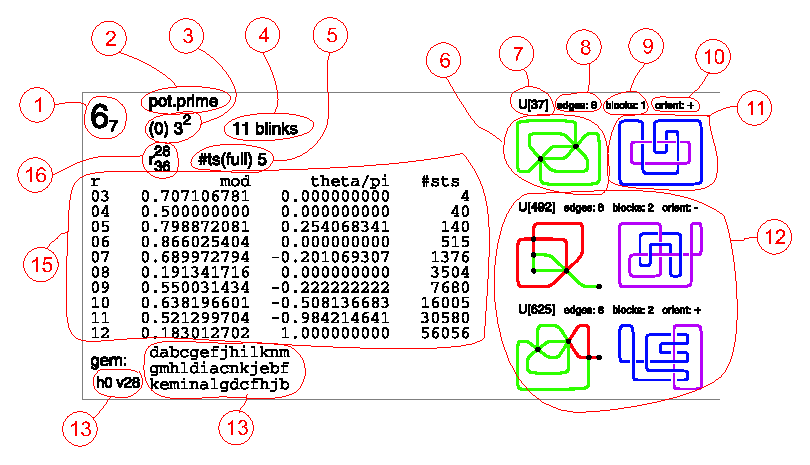
\includegraphics[width=14.5cm]{A.figs/catalogueexplanation.eps}
   \end{center}
   \vspace{-0.7cm}
   \caption{ Elements of catalogue}
   \label{fig:catalogueExplanation}
\end{figure}

The elements of this catalogue are: (1) the space name: $6_7$ is
a synonym for $6.7$; (2) the primality test outcome; (3) the homology
group; (4) the number of g-blinks in $U$ that induces this space; (5) number
of 3-gems identified in the same ts-class of the minimum 3-gem
found for this space: {\it full} means that all ts-class
was identified, {\it partial} means that we do not know if
all ts-class was identified; (6) the minimum blink
presentation for this space in set $U$ and also a
minimal presentation for this space (this is always true,
except for class $6.5$ that should be $0.1$); (7) the name
of the g-blink in $U$; (8) its number of edges; (9) its number
of blocks in the blink presentation (2-connected components);
(10) its orientation compared to the orientation of the QI shown:
+ sign means the same and - sign means different; (11) the
corresponding BFL presentation; (12) other g-blinks in the
same space; (13) the code of the minimal 3-gem found for
this space the code convention is defined in \cite{Lins1995};
 (14) the number of handles (composition with
$S^2 \times S^1$ and the number of vertices of this 3-gem); (15)
the quantum invariant of this space in polar form where the
angle is divided by $\pi$; (16) the name of this minimal
3-gem in the catalogue of \cite{Lins1995} when it is present
in this catalogue.

The spaces that have integral quantum invariants up to level 12 are:
6.5 $(S^2 \times S^1)$, 6.8, 6.18 and 8.32. The spaces that have real but not integral
quantum invariant up to level 12 are 1.1, 2.1, 4.4, 6.14, 6.19, 8.58,
8.70, 8.75, 8.76, 8.81, 8.86, 8.87, 8.89, 8.100, 8.102, 8.103, 8.117,
9.23, 9.183. The remaining classes have entries with non-zero imaginary
part (i.e. $\theta/\pi \notin \{0, 1\}$).



\begin{center}
 \includegraphics[height=23.5cm]{E.figsbw2/catalog001_bw.pdf} \eject
 \includegraphics[height=23.5cm]{E.figsbw2/catalog002_bw.pdf} \eject
 \includegraphics[height=23.5cm]{E.figsbw2/catalog003_bw.pdf} \eject
 \includegraphics[height=23.5cm]{E.figsbw2/catalog004_bw.pdf} \eject
 \includegraphics[height=23.5cm]{E.figsbw2/catalog005_bw.pdf} \eject
 \includegraphics[height=23.5cm]{E.figsbw2/catalog006_bw.pdf} \eject
 \includegraphics[height=23.5cm]{E.figsbw2/catalog007_bw.pdf} \eject
 \includegraphics[height=23.5cm]{E.figsbw2/catalog008_bw.pdf} \eject
 \includegraphics[height=23.5cm]{E.figsbw2/catalog009_bw.pdf} \eject
 \includegraphics[height=23.5cm]{E.figsbw2/catalog010_bw.pdf} \eject
 \includegraphics[height=23.5cm]{E.figsbw2/catalog011_bw.pdf} \eject
 \includegraphics[height=23.5cm]{E.figsbw2/catalog012_bw.pdf} \eject
 \includegraphics[height=23.5cm]{E.figsbw2/catalog013_bw.pdf} \eject
 \includegraphics[height=23.5cm]{E.figsbw2/catalog014_bw.pdf} \eject
 \includegraphics[height=23.5cm]{E.figsbw2/catalog015_bw.pdf} \eject
 \includegraphics[height=23.5cm]{E.figsbw2/catalog016_bw.pdf} \eject
 \includegraphics[height=23.5cm]{E.figsbw2/catalog017_bw.pdf} \eject
 \includegraphics[height=23.5cm]{E.figsbw2/catalog018_bw.pdf} \eject
 \includegraphics[height=23.5cm]{E.figsbw2/catalog019_bw.pdf} \eject
 \includegraphics[height=23.5cm]{E.figsbw2/catalog020_bw.pdf} \eject
 \includegraphics[height=23.5cm]{E.figsbw2/catalog021_bw.pdf} \eject
 \includegraphics[height=23.5cm]{E.figsbw2/catalog022_bw.pdf} \eject
 \includegraphics[height=23.5cm]{E.figsbw2/catalog023_bw.pdf} \eject
 \includegraphics[height=23.5cm]{E.figsbw2/catalog024_bw.pdf} \eject
 \includegraphics[height=23.5cm]{E.figsbw2/catalog025_bw.pdf} \eject
 \includegraphics[height=23.5cm]{E.figsbw2/catalog026_bw.pdf} \eject
 \includegraphics[height=23.5cm]{E.figsbw2/catalog027_bw.pdf} \eject
 \includegraphics[height=23.5cm]{E.figsbw2/catalog028_bw.pdf} \eject
 \includegraphics[height=23.5cm]{E.figsbw2/catalog029_bw.pdf} \eject
 \includegraphics[height=23.5cm]{E.figsbw2/catalog030_bw.pdf} \eject
 \includegraphics[height=23.5cm]{E.figsbw2/catalog031_bw.pdf} \eject
 \includegraphics[height=23.5cm]{E.figsbw2/catalog032_bw.pdf} \eject
 \includegraphics[height=23.5cm]{E.figsbw2/catalog033_bw.pdf} \eject
 \includegraphics[height=23.5cm]{E.figsbw2/catalog034_bw.pdf} \eject
 \includegraphics[height=23.5cm]{E.figsbw2/catalog035_bw.pdf} \eject
 \includegraphics[height=23.5cm]{E.figsbw2/catalog036_bw.pdf} \eject
 \includegraphics[height=23.5cm]{E.figsbw2/catalog037_bw.pdf} \eject
 \includegraphics[height=23.5cm]{E.figsbw2/catalog038_bw.pdf} \eject
 \includegraphics[height=23.5cm]{E.figsbw2/catalog039_bw.pdf} \eject
 \includegraphics[height=23.5cm]{E.figsbw2/catalog040_bw.pdf} \eject
 \includegraphics[height=23.5cm]{E.figsbw2/catalog041_bw.pdf} \eject
 \includegraphics[height=23.5cm]{E.figsbw2/catalog042_bw.pdf} \eject
 \includegraphics[height=23.5cm]{E.figsbw2/catalog043_bw.pdf} \eject
 \includegraphics[height=23.5cm]{E.figsbw2/catalog044_bw.pdf} \eject
 \includegraphics[height=23.5cm]{E.figsbw2/catalog045_bw.pdf} \eject
 \includegraphics[height=23.5cm]{E.figsbw2/catalog046_bw.pdf} \eject
 \includegraphics[height=23.5cm]{E.figsbw2/catalog047_bw.pdf} \eject
 \includegraphics[height=23.5cm]{E.figsbw2/catalog048_bw.pdf} \eject
 \includegraphics[height=23.5cm]{E.figsbw2/catalog049_bw.pdf} \eject
 \includegraphics[height=23.5cm]{E.figsbw2/catalog050_bw.pdf} \eject
 \includegraphics[height=23.5cm]{E.figsbw2/catalog051_bw.pdf} \eject
 \includegraphics[height=23.5cm]{E.figsbw2/catalog052_bw.pdf} \eject
 \includegraphics[height=23.5cm]{E.figsbw2/catalog053_bw.pdf} \eject
 \includegraphics[height=23.5cm]{E.figsbw2/catalog054_bw.pdf} \eject
 \includegraphics[height=23.5cm]{E.figsbw2/catalog055_bw.pdf} \eject
 \includegraphics[height=23.5cm]{E.figsbw2/catalog056_bw.pdf} \eject
 \includegraphics[height=23.5cm]{E.figsbw2/catalog057_bw.pdf} \eject
 \includegraphics[height=23.5cm]{E.figsbw2/catalog058_bw.pdf} \eject
 \includegraphics[height=23.5cm]{E.figsbw2/catalog059_bw.pdf} \eject
 \includegraphics[height=23.5cm]{E.figsbw2/catalog060_bw.pdf} \eject
 \includegraphics[height=23.5cm]{E.figsbw2/catalog061_bw.pdf} \eject
 \includegraphics[height=23.5cm]{E.figsbw2/catalog062_bw.pdf} \eject
 \includegraphics[height=23.5cm]{E.figsbw2/catalog063_bw.pdf} \eject
 \includegraphics[height=23.5cm]{E.figsbw2/catalog064_bw.pdf} \eject
 \includegraphics[height=23.5cm]{E.figsbw2/catalog065_bw.pdf} \eject
 \includegraphics[height=23.5cm]{E.figsbw2/catalog066_bw.pdf} \eject
 \includegraphics[height=23.5cm]{E.figsbw2/catalog067_bw.pdf} \eject
 \includegraphics[height=23.5cm]{E.figsbw2/catalog068_bw.pdf} \eject
 \includegraphics[height=23.5cm]{E.figsbw2/catalog069_bw.pdf} \eject
 \includegraphics[height=23.5cm]{E.figsbw2/catalog070_bw.pdf} \eject
 \includegraphics[height=23.5cm]{E.figsbw2/catalog071_bw.pdf} \eject
 \includegraphics[height=23.5cm]{E.figsbw2/catalog072_bw.pdf} \eject
 \includegraphics[height=23.5cm]{E.figsbw2/catalog073_bw.pdf} \eject
 \includegraphics[height=23.5cm]{E.figsbw2/catalog074_bw.pdf} \eject
 \includegraphics[height=23.5cm]{E.figsbw2/catalog075_bw.pdf} \eject
 \includegraphics[height=23.5cm]{E.figsbw2/catalog076_bw.pdf} \eject
 \includegraphics[height=23.5cm]{E.figsbw2/catalog077_bw.pdf} \eject
 \includegraphics[height=23.5cm]{E.figsbw2/catalog078_bw.pdf} \eject
 \includegraphics[height=23.5cm]{E.figsbw2/catalog079_bw.pdf} \eject
 \includegraphics[height=23.5cm]{E.figsbw2/catalog080_bw.pdf} \eject
 \includegraphics[height=23.5cm]{E.figsbw2/catalog081_bw.pdf} \eject
 \includegraphics[height=23.5cm]{E.figsbw2/catalog082_bw.pdf} \eject
 \includegraphics[height=23.5cm]{E.figsbw2/catalog083_bw.pdf} \eject
 \includegraphics[height=23.5cm]{E.figsbw2/catalog084_bw.pdf} \eject
 \includegraphics[height=23.5cm]{E.figsbw2/catalog085_bw.pdf} \eject
 \includegraphics[height=23.5cm]{E.figsbw2/catalog086_bw.pdf} \eject
 \includegraphics[height=23.5cm]{E.figsbw2/catalog087_bw.pdf} \eject
 \includegraphics[height=23.5cm]{E.figsbw2/catalog088_bw.pdf} \eject
 \includegraphics[height=23.5cm]{E.figsbw2/catalog089_bw.pdf} \eject
 \includegraphics[height=23.5cm]{E.figsbw2/catalog090_bw.pdf} \eject
 \includegraphics[height=23.5cm]{E.figsbw2/catalog091_bw.pdf} \eject
 \includegraphics[height=23.5cm]{E.figsbw2/catalog092_bw.pdf} \eject
 \includegraphics[height=23.5cm]{E.figsbw2/catalog093_bw.pdf} \eject
 \includegraphics[height=23.5cm]{E.figsbw2/catalog094_bw.pdf} \eject
 \includegraphics[height=23.5cm]{E.figsbw2/catalog095_bw.pdf} \eject
 \includegraphics[height=23.5cm]{E.figsbw2/catalog096_bw.pdf} \eject
 \includegraphics[height=23.5cm]{E.figsbw2/catalog097_bw.pdf} \eject
 \includegraphics[height=23.5cm]{E.figsbw2/catalog098_bw.pdf} \eject
 \includegraphics[height=23.5cm]{E.figsbw2/catalog099_bw.pdf} \eject
 \includegraphics[height=23.5cm]{E.figsbw2/catalog100_bw.pdf} \eject 
 \includegraphics[height=23.5cm]{E.figsbw2/catalog101_bw.pdf} \eject
\end{center}




\section{Appendix: The 14 composite spaces in $U$}
\label{chap:compositeCatalogue}

We here present the 14 spaces induced from g-blinks in $U$.
Their ``connected sum'' details: what prime spaces compose to
them are shown in Chapter~\ref{chap:census}. The elements of
this presentation are the same as the explained in
Appendix~\ref{chap:primeCatalogue}.

% \newcount\ii \newcount\jj   % declare integer variable
% \def\producePagesTwo#1#2{
% \ii=#1                      % initialize ii
% \jj=#2                      % initialize jj
% \advance\jj by 1            % increment jj
% \loop   % loop
%    \ifnum\ii<\jj
% {
%    %\vspace{-1cm}
%    %\thispagestyle{empty}
%    % \setlength{\hoffset}{0cm}
%    % \setlength{\textwidth}{\paperwidth-2cm}
%    \hspace{-1.8cm}
%    \enlargethispage{5cm}
%    {\centering
%    \includegraphics[height=23.5cm]{A.figs/compcatalog\ifnum\ii<100 0\fi\ifnum\ii<10 0\fi\number\ii.eps}
%    }
%    \newpage}
%       \advance\ii by 1
%    \repeat
% }

\newpage
\setlength{\topmargin}{-1.2cm}
%\setlength{\textwidth}{\paperwidth-2in}
%\setlength{\headheight}{1cm}
%\setlength{\headsep}{-3cm}
%\setlength{\footskip}{0.1cm}
%\setlength{\textheight}{\paperheight-\headheight-\headsep-\footskip-2in}
%\setlength{\oddsidemargin}{0mm}
%\setlength{\evensidemargin}{0mm}
%\setlength{\marginparwidth}{0mm}
%\setlength{\marginparsep}{0mm}
%\setlength{\textwidth}{\paperwidth-2in}

\begin{center}
 \includegraphics[height=23.5cm]{E.figsbw2/compcatalog001_bw.pdf} \eject
 \includegraphics[height=23.5cm]{E.figsbw2/compcatalog002_bw.pdf} \eject 
 \includegraphics[height=23.5cm]{E.figsbw2/compcatalog003_bw.pdf} \eject
\end{center}
\section{Appendix: Simple 3-connected monochromatic blinks up to 16 edges}
\label{chap:catalolgue3con}

We here present all simple 3-connected green blinks with
$\leq 16$ edges divided in 381 HGnQI classes. The quantum
invariant was calculated up to level $r=8$ for each of
these blinks. There are left 11 uncertainties: 14.24t,
15.16t, 15.19t, 15.22t, 16.42t, 16.56t, 16.141t, 16.142t,
16.149t, 16.233t. Except for these classes the other 370
consisted of only one blink (or the two orientations of
the same space). This fact suggests that if $A$ and $B$
are two different simple 3-connected monochromatic blinks,
that do not form a trivial pair (trivially induce the
same space), then they probably induce different spaces.
Are the 11 uncertainties examples of non-trivial pairs?

\begin{center}
\includegraphics{A.figs/doubts3connectedisolated.eps}
\end{center}

\setlength{\topmargin}{-1.2cm}
%\setlength{\textwidth}{\paperwidth-2in}
%\setlength{\headheight}{1cm}
%\setlength{\headsep}{-3cm}
%\setlength{\footskip}{0.1cm}
%\setlength{\textheight}{\paperheight-\headheight-\headsep-\footskip-2in}
%\setlength{\oddsidemargin}{0mm}
%\setlength{\evensidemargin}{0mm}
%\setlength{\marginparwidth}{0mm}
%\setlength{\marginparsep}{0mm}
%\setlength{\textwidth}{\paperwidth-2in}

\begin{center}
 \includegraphics[height=23.5cm]{E.figsbw2/con3catalog001_bw.pdf} \eject
 \includegraphics[height=23.5cm]{E.figsbw2/con3catalog002_bw.pdf} \eject
 \includegraphics[height=23.5cm]{E.figsbw2/con3catalog003_bw.pdf} \eject
 \includegraphics[height=23.5cm]{E.figsbw2/con3catalog004_bw.pdf} \eject 
 \includegraphics[height=23.5cm]{E.figsbw2/con3catalog005_bw.pdf} \eject
 \includegraphics[height=23.5cm]{E.figsbw2/con3catalog006_bw.pdf} \eject
 \includegraphics[height=23.5cm]{E.figsbw2/con3catalog007_bw.pdf} \eject
 \includegraphics[height=23.5cm]{E.figsbw2/con3catalog008_bw.pdf} \eject 
 \includegraphics[height=23.5cm]{E.figsbw2/con3catalog009_bw.pdf} \eject
 \includegraphics[height=23.5cm]{E.figsbw2/con3catalog010_bw.pdf} \eject
 \includegraphics[height=23.5cm]{E.figsbw2/con3catalog011_bw.pdf} \eject
 \includegraphics[height=23.5cm]{E.figsbw2/con3catalog012_bw.pdf} \eject 
 \includegraphics[height=23.5cm]{E.figsbw2/con3catalog013_bw.pdf} \eject
 \includegraphics[height=23.5cm]{E.figsbw2/con3catalog014_bw.pdf} \eject
 \includegraphics[height=23.5cm]{E.figsbw2/con3catalog015_bw.pdf} \eject
 \includegraphics[height=23.5cm]{E.figsbw2/con3catalog016_bw.pdf} \eject  
 \includegraphics[height=23.5cm]{E.figsbw2/con3catalog017_bw.pdf} \eject
 \includegraphics[height=23.5cm]{E.figsbw2/con3catalog018_bw.pdf} \eject
 \includegraphics[height=23.5cm]{E.figsbw2/con3catalog019_bw.pdf} \eject
 \includegraphics[height=23.5cm]{E.figsbw2/con3catalog020_bw.pdf} \eject 
 \includegraphics[height=23.5cm]{E.figsbw2/con3catalog021_bw.pdf} \eject
 \includegraphics[height=23.5cm]{E.figsbw2/con3catalog022_bw.pdf} \eject
 \includegraphics[height=23.5cm]{E.figsbw2/con3catalog023_bw.pdf} \eject
 \includegraphics[height=23.5cm]{E.figsbw2/con3catalog024_bw.pdf} \eject 
 \includegraphics[height=23.5cm]{E.figsbw2/con3catalog025_bw.pdf} \eject
 \includegraphics[height=23.5cm]{E.figsbw2/con3catalog026_bw.pdf} \eject
 \includegraphics[height=23.5cm]{E.figsbw2/con3catalog027_bw.pdf} \eject
 \includegraphics[height=23.5cm]{E.figsbw2/con3catalog028_bw.pdf} \eject 
 \includegraphics[height=23.5cm]{E.figsbw2/con3catalog029_bw.pdf} \eject
 \includegraphics[height=23.5cm]{E.figsbw2/con3catalog030_bw.pdf} \eject
 \includegraphics[height=23.5cm]{E.figsbw2/con3catalog031_bw.pdf} \eject
 \includegraphics[height=23.5cm]{E.figsbw2/con3catalog032_bw.pdf} \eject  
 \includegraphics[height=23.5cm]{E.figsbw2/con3catalog033_bw.pdf} \eject
 \includegraphics[height=23.5cm]{E.figsbw2/con3catalog034_bw.pdf} \eject  
 \includegraphics[height=23.5cm]{E.figsbw2/con3catalog035_bw.pdf} \eject
 \includegraphics[height=23.5cm]{E.figsbw2/con3catalog036_bw.pdf} \eject  
 \includegraphics[height=23.5cm]{E.figsbw2/con3catalog037_bw.pdf} \eject
 \includegraphics[height=23.5cm]{E.figsbw2/con3catalog038_bw.pdf} \eject  
 \includegraphics[height=23.5cm]{E.figsbw2/con3catalog039_bw.pdf} \eject
\end{center}
 
% \newcount\ii \newcount\jj   % declare integer variable
% \def\producePagesThree#1#2{
% \ii=#1                      % initialize ii
% \jj=#2                      % initialize jj
% \advance\jj by 1            % increment jj
% \loop   % loop
%    \ifnum\ii<\jj
% {
%    %\vspace{-1cm}
%    %\thispagestyle{empty}
%    % \setlength{\hoffset}{0cm}
%    % \setlength{\textwidth}{\paperwidth-2cm}
%    \hspace{-1.8cm}
%    \enlargethispage{5cm}
%    {\centering
%    \includegraphics[height=23.5cm]{E.figsbw2/con3catalog\ifnum\ii<100 0\fi\ifnum\ii<10 0\fi\number\ii.eps}
%    }
%    \newpage}
%       \advance\ii by 1
%    \repeat
% }


%\newlength{\topmarginOne}
%\setlength{\topmarginOne}{\topmargin}
%\setlength{\topmargin}{\topmarginOne}


% � aconselh�vel criar cada ap�ndice em um arquivo � parte, digamos
% "apendice1.tex", "apendice.tex", ... "apendiceM.tex" e depois
% inclu�-los com:
% 
\section{The 487 potentially prime spaces in $U$}
\label{chap:primeCatalogue}

We present in this chapter the 487 spaces that are ``potentially prime'' once we could
not prove them composite in our tests. One thing is certain, as stated in
Theorem~\ref{theo:primeSpacesUpTo9Edges}: any prime space that can be
presented as a blink with $\leq$ 9 edges induces the same space (modulo
orientation) as one and only one of these 487 spaces. Actually there
are two points where this last statement may fail: space 9.126 and space 9.199 (although
they have the same HGnQI we could not find a proof of homeomorphism
between g-blink $U[1563]$ and the other g-blinks in 9.126 and g-blink $U[2165]$
and the others in 9.199). All 3437 g-blinks in $U$ appears in this Appendix or
in Appendix~\ref{chap:compositeCatalogue}.

\begin{figure}[htp]
   \begin{center}
      \leavevmode
      \includegraphics[width=14.5cm]{A.figs/catalogueexplanation.eps}
   \end{center}
   \vspace{-0.7cm}
   \caption{ Elements of catalogue}
   \label{fig:catalogueExplanation}
\end{figure}

The elements of this catalogue are: (1) the space name: $6_7$ is
a synonym for $6.7$; (2) the primality test outcome; (3) the homology
group; (4) the number of g-blinks in $U$ that induces this space; (5) number
of 3-gems identified in the same ts-class of the minimum 3-gem
found for this space: {\it full} means that all ts-class
was identified, {\it partial} means that we do not know if
all ts-class was identified; (6) the minimum blink
presentation for this space in set $U$ and also a
minimal presentation for this space (this is always true,
except for class $6.5$ that should be $0.1$); (7) the name
of the g-blink in $U$; (8) its number of edges; (9) its number
of blocks in the blink presentation (2-connected components);
(10) its orientation compared to the orientation of the QI shown:
+ sign means the same and - sign means different; (11) the
corresponding BFL presentation; (12) other g-blinks in the
same space; (13) the code of the minimal 3-gem found for
this space the code convention is defined in \cite{Lins1995};
 (14) the number of handles (composition with
$S^2 \times S^1$ and the number of vertices of this 3-gem); (15)
the quantum invariant of this space in polar form where the
angle is divided by $\pi$; (16) the name of this minimal
3-gem in the catalogue of \cite{Lins1995} when it is present
in this catalogue.

The spaces that have integral quantum invariants up to level 12 are:
6.5 $(S^2 \times S^1)$, 6.8, 6.18 and 8.32. The spaces that have real but not integral
quantum invariant up to level 12 are 1.1, 2.1, 4.4, 6.14, 6.19, 8.58,
8.70, 8.75, 8.76, 8.81, 8.86, 8.87, 8.89, 8.100, 8.102, 8.103, 8.117,
9.23, 9.183. The remaining classes have entries with non-zero imaginary
part (i.e. $\theta/\pi \notin \{0, 1\}$).



\begin{center}
 \includegraphics[height=23.5cm]{E.figsbw2/catalog001_bw.pdf} \eject
 \includegraphics[height=23.5cm]{E.figsbw2/catalog002_bw.pdf} \eject
 \includegraphics[height=23.5cm]{E.figsbw2/catalog003_bw.pdf} \eject
 \includegraphics[height=23.5cm]{E.figsbw2/catalog004_bw.pdf} \eject
 \includegraphics[height=23.5cm]{E.figsbw2/catalog005_bw.pdf} \eject
 \includegraphics[height=23.5cm]{E.figsbw2/catalog006_bw.pdf} \eject
 \includegraphics[height=23.5cm]{E.figsbw2/catalog007_bw.pdf} \eject
 \includegraphics[height=23.5cm]{E.figsbw2/catalog008_bw.pdf} \eject
 \includegraphics[height=23.5cm]{E.figsbw2/catalog009_bw.pdf} \eject
 \includegraphics[height=23.5cm]{E.figsbw2/catalog010_bw.pdf} \eject
 \includegraphics[height=23.5cm]{E.figsbw2/catalog011_bw.pdf} \eject
 \includegraphics[height=23.5cm]{E.figsbw2/catalog012_bw.pdf} \eject
 \includegraphics[height=23.5cm]{E.figsbw2/catalog013_bw.pdf} \eject
 \includegraphics[height=23.5cm]{E.figsbw2/catalog014_bw.pdf} \eject
 \includegraphics[height=23.5cm]{E.figsbw2/catalog015_bw.pdf} \eject
 \includegraphics[height=23.5cm]{E.figsbw2/catalog016_bw.pdf} \eject
 \includegraphics[height=23.5cm]{E.figsbw2/catalog017_bw.pdf} \eject
 \includegraphics[height=23.5cm]{E.figsbw2/catalog018_bw.pdf} \eject
 \includegraphics[height=23.5cm]{E.figsbw2/catalog019_bw.pdf} \eject
 \includegraphics[height=23.5cm]{E.figsbw2/catalog020_bw.pdf} \eject
 \includegraphics[height=23.5cm]{E.figsbw2/catalog021_bw.pdf} \eject
 \includegraphics[height=23.5cm]{E.figsbw2/catalog022_bw.pdf} \eject
 \includegraphics[height=23.5cm]{E.figsbw2/catalog023_bw.pdf} \eject
 \includegraphics[height=23.5cm]{E.figsbw2/catalog024_bw.pdf} \eject
 \includegraphics[height=23.5cm]{E.figsbw2/catalog025_bw.pdf} \eject
 \includegraphics[height=23.5cm]{E.figsbw2/catalog026_bw.pdf} \eject
 \includegraphics[height=23.5cm]{E.figsbw2/catalog027_bw.pdf} \eject
 \includegraphics[height=23.5cm]{E.figsbw2/catalog028_bw.pdf} \eject
 \includegraphics[height=23.5cm]{E.figsbw2/catalog029_bw.pdf} \eject
 \includegraphics[height=23.5cm]{E.figsbw2/catalog030_bw.pdf} \eject
 \includegraphics[height=23.5cm]{E.figsbw2/catalog031_bw.pdf} \eject
 \includegraphics[height=23.5cm]{E.figsbw2/catalog032_bw.pdf} \eject
 \includegraphics[height=23.5cm]{E.figsbw2/catalog033_bw.pdf} \eject
 \includegraphics[height=23.5cm]{E.figsbw2/catalog034_bw.pdf} \eject
 \includegraphics[height=23.5cm]{E.figsbw2/catalog035_bw.pdf} \eject
 \includegraphics[height=23.5cm]{E.figsbw2/catalog036_bw.pdf} \eject
 \includegraphics[height=23.5cm]{E.figsbw2/catalog037_bw.pdf} \eject
 \includegraphics[height=23.5cm]{E.figsbw2/catalog038_bw.pdf} \eject
 \includegraphics[height=23.5cm]{E.figsbw2/catalog039_bw.pdf} \eject
 \includegraphics[height=23.5cm]{E.figsbw2/catalog040_bw.pdf} \eject
 \includegraphics[height=23.5cm]{E.figsbw2/catalog041_bw.pdf} \eject
 \includegraphics[height=23.5cm]{E.figsbw2/catalog042_bw.pdf} \eject
 \includegraphics[height=23.5cm]{E.figsbw2/catalog043_bw.pdf} \eject
 \includegraphics[height=23.5cm]{E.figsbw2/catalog044_bw.pdf} \eject
 \includegraphics[height=23.5cm]{E.figsbw2/catalog045_bw.pdf} \eject
 \includegraphics[height=23.5cm]{E.figsbw2/catalog046_bw.pdf} \eject
 \includegraphics[height=23.5cm]{E.figsbw2/catalog047_bw.pdf} \eject
 \includegraphics[height=23.5cm]{E.figsbw2/catalog048_bw.pdf} \eject
 \includegraphics[height=23.5cm]{E.figsbw2/catalog049_bw.pdf} \eject
 \includegraphics[height=23.5cm]{E.figsbw2/catalog050_bw.pdf} \eject
 \includegraphics[height=23.5cm]{E.figsbw2/catalog051_bw.pdf} \eject
 \includegraphics[height=23.5cm]{E.figsbw2/catalog052_bw.pdf} \eject
 \includegraphics[height=23.5cm]{E.figsbw2/catalog053_bw.pdf} \eject
 \includegraphics[height=23.5cm]{E.figsbw2/catalog054_bw.pdf} \eject
 \includegraphics[height=23.5cm]{E.figsbw2/catalog055_bw.pdf} \eject
 \includegraphics[height=23.5cm]{E.figsbw2/catalog056_bw.pdf} \eject
 \includegraphics[height=23.5cm]{E.figsbw2/catalog057_bw.pdf} \eject
 \includegraphics[height=23.5cm]{E.figsbw2/catalog058_bw.pdf} \eject
 \includegraphics[height=23.5cm]{E.figsbw2/catalog059_bw.pdf} \eject
 \includegraphics[height=23.5cm]{E.figsbw2/catalog060_bw.pdf} \eject
 \includegraphics[height=23.5cm]{E.figsbw2/catalog061_bw.pdf} \eject
 \includegraphics[height=23.5cm]{E.figsbw2/catalog062_bw.pdf} \eject
 \includegraphics[height=23.5cm]{E.figsbw2/catalog063_bw.pdf} \eject
 \includegraphics[height=23.5cm]{E.figsbw2/catalog064_bw.pdf} \eject
 \includegraphics[height=23.5cm]{E.figsbw2/catalog065_bw.pdf} \eject
 \includegraphics[height=23.5cm]{E.figsbw2/catalog066_bw.pdf} \eject
 \includegraphics[height=23.5cm]{E.figsbw2/catalog067_bw.pdf} \eject
 \includegraphics[height=23.5cm]{E.figsbw2/catalog068_bw.pdf} \eject
 \includegraphics[height=23.5cm]{E.figsbw2/catalog069_bw.pdf} \eject
 \includegraphics[height=23.5cm]{E.figsbw2/catalog070_bw.pdf} \eject
 \includegraphics[height=23.5cm]{E.figsbw2/catalog071_bw.pdf} \eject
 \includegraphics[height=23.5cm]{E.figsbw2/catalog072_bw.pdf} \eject
 \includegraphics[height=23.5cm]{E.figsbw2/catalog073_bw.pdf} \eject
 \includegraphics[height=23.5cm]{E.figsbw2/catalog074_bw.pdf} \eject
 \includegraphics[height=23.5cm]{E.figsbw2/catalog075_bw.pdf} \eject
 \includegraphics[height=23.5cm]{E.figsbw2/catalog076_bw.pdf} \eject
 \includegraphics[height=23.5cm]{E.figsbw2/catalog077_bw.pdf} \eject
 \includegraphics[height=23.5cm]{E.figsbw2/catalog078_bw.pdf} \eject
 \includegraphics[height=23.5cm]{E.figsbw2/catalog079_bw.pdf} \eject
 \includegraphics[height=23.5cm]{E.figsbw2/catalog080_bw.pdf} \eject
 \includegraphics[height=23.5cm]{E.figsbw2/catalog081_bw.pdf} \eject
 \includegraphics[height=23.5cm]{E.figsbw2/catalog082_bw.pdf} \eject
 \includegraphics[height=23.5cm]{E.figsbw2/catalog083_bw.pdf} \eject
 \includegraphics[height=23.5cm]{E.figsbw2/catalog084_bw.pdf} \eject
 \includegraphics[height=23.5cm]{E.figsbw2/catalog085_bw.pdf} \eject
 \includegraphics[height=23.5cm]{E.figsbw2/catalog086_bw.pdf} \eject
 \includegraphics[height=23.5cm]{E.figsbw2/catalog087_bw.pdf} \eject
 \includegraphics[height=23.5cm]{E.figsbw2/catalog088_bw.pdf} \eject
 \includegraphics[height=23.5cm]{E.figsbw2/catalog089_bw.pdf} \eject
 \includegraphics[height=23.5cm]{E.figsbw2/catalog090_bw.pdf} \eject
 \includegraphics[height=23.5cm]{E.figsbw2/catalog091_bw.pdf} \eject
 \includegraphics[height=23.5cm]{E.figsbw2/catalog092_bw.pdf} \eject
 \includegraphics[height=23.5cm]{E.figsbw2/catalog093_bw.pdf} \eject
 \includegraphics[height=23.5cm]{E.figsbw2/catalog094_bw.pdf} \eject
 \includegraphics[height=23.5cm]{E.figsbw2/catalog095_bw.pdf} \eject
 \includegraphics[height=23.5cm]{E.figsbw2/catalog096_bw.pdf} \eject
 \includegraphics[height=23.5cm]{E.figsbw2/catalog097_bw.pdf} \eject
 \includegraphics[height=23.5cm]{E.figsbw2/catalog098_bw.pdf} \eject
 \includegraphics[height=23.5cm]{E.figsbw2/catalog099_bw.pdf} \eject
 \includegraphics[height=23.5cm]{E.figsbw2/catalog100_bw.pdf} \eject 
 \includegraphics[height=23.5cm]{E.figsbw2/catalog101_bw.pdf} \eject
\end{center}




% \section{Appendix: The 14 composite spaces in $U$}
\label{chap:compositeCatalogue}

We here present the 14 spaces induced from g-blinks in $U$.
Their ``connected sum'' details: what prime spaces compose to
them are shown in Chapter~\ref{chap:census}. The elements of
this presentation are the same as the explained in
Appendix~\ref{chap:primeCatalogue}.

% \newcount\ii \newcount\jj   % declare integer variable
% \def\producePagesTwo#1#2{
% \ii=#1                      % initialize ii
% \jj=#2                      % initialize jj
% \advance\jj by 1            % increment jj
% \loop   % loop
%    \ifnum\ii<\jj
% {
%    %\vspace{-1cm}
%    %\thispagestyle{empty}
%    % \setlength{\hoffset}{0cm}
%    % \setlength{\textwidth}{\paperwidth-2cm}
%    \hspace{-1.8cm}
%    \enlargethispage{5cm}
%    {\centering
%    \includegraphics[height=23.5cm]{A.figs/compcatalog\ifnum\ii<100 0\fi\ifnum\ii<10 0\fi\number\ii.eps}
%    }
%    \newpage}
%       \advance\ii by 1
%    \repeat
% }

\newpage
\setlength{\topmargin}{-1.2cm}
%\setlength{\textwidth}{\paperwidth-2in}
%\setlength{\headheight}{1cm}
%\setlength{\headsep}{-3cm}
%\setlength{\footskip}{0.1cm}
%\setlength{\textheight}{\paperheight-\headheight-\headsep-\footskip-2in}
%\setlength{\oddsidemargin}{0mm}
%\setlength{\evensidemargin}{0mm}
%\setlength{\marginparwidth}{0mm}
%\setlength{\marginparsep}{0mm}
%\setlength{\textwidth}{\paperwidth-2in}

\begin{center}
 \includegraphics[height=23.5cm]{E.figsbw2/compcatalog001_bw.pdf} \eject
 \includegraphics[height=23.5cm]{E.figsbw2/compcatalog002_bw.pdf} \eject 
 \includegraphics[height=23.5cm]{E.figsbw2/compcatalog003_bw.pdf} \eject
\end{center}
% \section{Appendix: Simple 3-connected monochromatic blinks up to 16 edges}
\label{chap:catalolgue3con}

We here present all simple 3-connected green blinks with
$\leq 16$ edges divided in 381 HGnQI classes. The quantum
invariant was calculated up to level $r=8$ for each of
these blinks. There are left 11 uncertainties: 14.24t,
15.16t, 15.19t, 15.22t, 16.42t, 16.56t, 16.141t, 16.142t,
16.149t, 16.233t. Except for these classes the other 370
consisted of only one blink (or the two orientations of
the same space). This fact suggests that if $A$ and $B$
are two different simple 3-connected monochromatic blinks,
that do not form a trivial pair (trivially induce the
same space), then they probably induce different spaces.
Are the 11 uncertainties examples of non-trivial pairs?

\begin{center}
\includegraphics{A.figs/doubts3connectedisolated.eps}
\end{center}

\setlength{\topmargin}{-1.2cm}
%\setlength{\textwidth}{\paperwidth-2in}
%\setlength{\headheight}{1cm}
%\setlength{\headsep}{-3cm}
%\setlength{\footskip}{0.1cm}
%\setlength{\textheight}{\paperheight-\headheight-\headsep-\footskip-2in}
%\setlength{\oddsidemargin}{0mm}
%\setlength{\evensidemargin}{0mm}
%\setlength{\marginparwidth}{0mm}
%\setlength{\marginparsep}{0mm}
%\setlength{\textwidth}{\paperwidth-2in}

\begin{center}
 \includegraphics[height=23.5cm]{E.figsbw2/con3catalog001_bw.pdf} \eject
 \includegraphics[height=23.5cm]{E.figsbw2/con3catalog002_bw.pdf} \eject
 \includegraphics[height=23.5cm]{E.figsbw2/con3catalog003_bw.pdf} \eject
 \includegraphics[height=23.5cm]{E.figsbw2/con3catalog004_bw.pdf} \eject 
 \includegraphics[height=23.5cm]{E.figsbw2/con3catalog005_bw.pdf} \eject
 \includegraphics[height=23.5cm]{E.figsbw2/con3catalog006_bw.pdf} \eject
 \includegraphics[height=23.5cm]{E.figsbw2/con3catalog007_bw.pdf} \eject
 \includegraphics[height=23.5cm]{E.figsbw2/con3catalog008_bw.pdf} \eject 
 \includegraphics[height=23.5cm]{E.figsbw2/con3catalog009_bw.pdf} \eject
 \includegraphics[height=23.5cm]{E.figsbw2/con3catalog010_bw.pdf} \eject
 \includegraphics[height=23.5cm]{E.figsbw2/con3catalog011_bw.pdf} \eject
 \includegraphics[height=23.5cm]{E.figsbw2/con3catalog012_bw.pdf} \eject 
 \includegraphics[height=23.5cm]{E.figsbw2/con3catalog013_bw.pdf} \eject
 \includegraphics[height=23.5cm]{E.figsbw2/con3catalog014_bw.pdf} \eject
 \includegraphics[height=23.5cm]{E.figsbw2/con3catalog015_bw.pdf} \eject
 \includegraphics[height=23.5cm]{E.figsbw2/con3catalog016_bw.pdf} \eject  
 \includegraphics[height=23.5cm]{E.figsbw2/con3catalog017_bw.pdf} \eject
 \includegraphics[height=23.5cm]{E.figsbw2/con3catalog018_bw.pdf} \eject
 \includegraphics[height=23.5cm]{E.figsbw2/con3catalog019_bw.pdf} \eject
 \includegraphics[height=23.5cm]{E.figsbw2/con3catalog020_bw.pdf} \eject 
 \includegraphics[height=23.5cm]{E.figsbw2/con3catalog021_bw.pdf} \eject
 \includegraphics[height=23.5cm]{E.figsbw2/con3catalog022_bw.pdf} \eject
 \includegraphics[height=23.5cm]{E.figsbw2/con3catalog023_bw.pdf} \eject
 \includegraphics[height=23.5cm]{E.figsbw2/con3catalog024_bw.pdf} \eject 
 \includegraphics[height=23.5cm]{E.figsbw2/con3catalog025_bw.pdf} \eject
 \includegraphics[height=23.5cm]{E.figsbw2/con3catalog026_bw.pdf} \eject
 \includegraphics[height=23.5cm]{E.figsbw2/con3catalog027_bw.pdf} \eject
 \includegraphics[height=23.5cm]{E.figsbw2/con3catalog028_bw.pdf} \eject 
 \includegraphics[height=23.5cm]{E.figsbw2/con3catalog029_bw.pdf} \eject
 \includegraphics[height=23.5cm]{E.figsbw2/con3catalog030_bw.pdf} \eject
 \includegraphics[height=23.5cm]{E.figsbw2/con3catalog031_bw.pdf} \eject
 \includegraphics[height=23.5cm]{E.figsbw2/con3catalog032_bw.pdf} \eject  
 \includegraphics[height=23.5cm]{E.figsbw2/con3catalog033_bw.pdf} \eject
 \includegraphics[height=23.5cm]{E.figsbw2/con3catalog034_bw.pdf} \eject  
 \includegraphics[height=23.5cm]{E.figsbw2/con3catalog035_bw.pdf} \eject
 \includegraphics[height=23.5cm]{E.figsbw2/con3catalog036_bw.pdf} \eject  
 \includegraphics[height=23.5cm]{E.figsbw2/con3catalog037_bw.pdf} \eject
 \includegraphics[height=23.5cm]{E.figsbw2/con3catalog038_bw.pdf} \eject  
 \includegraphics[height=23.5cm]{E.figsbw2/con3catalog039_bw.pdf} \eject
\end{center}
 
% \newcount\ii \newcount\jj   % declare integer variable
% \def\producePagesThree#1#2{
% \ii=#1                      % initialize ii
% \jj=#2                      % initialize jj
% \advance\jj by 1            % increment jj
% \loop   % loop
%    \ifnum\ii<\jj
% {
%    %\vspace{-1cm}
%    %\thispagestyle{empty}
%    % \setlength{\hoffset}{0cm}
%    % \setlength{\textwidth}{\paperwidth-2cm}
%    \hspace{-1.8cm}
%    \enlargethispage{5cm}
%    {\centering
%    \includegraphics[height=23.5cm]{E.figsbw2/con3catalog\ifnum\ii<100 0\fi\ifnum\ii<10 0\fi\number\ii.eps}
%    }
%    \newpage}
%       \advance\ii by 1
%    \repeat
% }


%\newlength{\topmarginOne}
%\setlength{\topmarginOne}{\topmargin}
%\setlength{\topmargin}{\topmarginOne}

% ...
% \include{apendiceM}


% Bibliografia
% � aconselh�vel utilizar o BibTeX a partir de um arquivo, digamos "biblio.bib".
% Para ajuda na cria��o do arquivo .bib e utiliza��o do BibTeX, recorra ao
% BibTeXpress em www.cin.ufpe.br/~paguso/bibtexpress
\setlength{\topmargin}{0cm}
%\bibliographystyle{alpha}
%\nocite{*}
\bibliographystyle{plain}
\bibliography{bibtexIndex.bib}

% C�lofon
% Inclui uma pequena nota com refer�ncia � UFPEThesis
% Comente para omitir
%\colophon

%% Fim do documento
\end{document}
